\chapter{案例分析}
\section{案例實驗設計}\label{s4.1}
\indent
本論文提出的工具適用於畫面出現變化的情況,因此在實驗網站的挑選上,會以互動功能較多的網站為第一優先。
在眾多的模板網頁中,圖\ref{f4.1}所示的家具銷售模板網站\cite{Furn-Free-CSS-Template}符合互動多的特性,
因此本實驗的實驗網站以該網站為基礎來做修改。
本論文的實驗案例是基於撰寫測試腳本時常會遇到的情況下,
挑選出五個情境並設計成符合實驗網頁的情境來讓實驗人員實際操作。

\begin{figure}[H]
    \centering
    \setlength{\abovecaptionskip}{-5pt}
    \setlength{\belowcaptionskip}{0pt}
    \includegraphics[width=0.88\textwidth]{picture/experiment/test-environment-demo.png}
    \caption{實驗模板網站}
    \label{f4.1}
\end{figure}

在實驗人員的選擇的部分,
將以有資工相關背景為優先選擇並邀請到14位皆為臺北科技大學資工系的學生,
其中包含大二、大三的專題生和碩士一年級、二年級的同學,
並將它們分成七位有網頁測試相關經驗和七位對此技術較為陌生兩種類別的人。
為因應目前疫情時間,測試環境皆在同一台電腦進行操作,
實體操作則直接操作電腦,
遠端操作則使用Window遠端連線到該電腦來進行操作。
另外,為確保實體和遠端的操作環境相同,遠端設備皆會檢測網速在至少在100Mbps以上,並確保操作畫面時不會有遲鈍的現象。
操作的鍵盤滑鼠均使用實驗者平時在使用的設備,
實驗人員的操作介面為Chrome瀏覽器,工具為Chrome瀏覽器中的Developer Tools和本實驗提出的擴充元件。
在實驗過程中,會確保實驗人員在只有一個人的環境中進行案例實作以及排除任何會影響實驗準確性之外在因素,
例如:手機、通訊軟體、開啟其他瀏覽器分頁等等

實驗流程開始前,
會先對實驗人員用同一個簡報簡易說明該論文的背景知識、測試目的以及實驗網頁的簡單介紹,
之後會示範操作一個簡易的範例並且讓實驗人員親自操作此範例來熟悉該工具,
一切初始程序就位後才會開始操作實驗案例。
操作實驗案例的流程為先講解實作案例的情境,確認實驗人員了解後開始計時,直到實驗人員找出結果後才停止計時,
每位實驗人員皆會操作實驗章節\ref{s4.2}提到的五個實驗案例,
先以只使用Developer Tools的情況下實作五個實驗案例,
再以使用Developer Tools加上擴充元件的情況實作五個相同實驗案例。
等待14位實驗人員操作完成後,統整所有實驗人員的相關數據並以是否有使用本實驗提出擴充元件和是否有相關經驗兩種因素進行實作時間比較,

\section{測試案例實作}\label{s4.2}

\subsection{案例一:Hover購物車圖示後出現購物車下拉式畫面}\label{s4.2.1}
\indent
實驗人員的測試情境為將滑鼠放在購物車的圖示上,
等到下拉式畫面出現後,需要找出所有因為下拉式畫面出現而屬性變化的元件,如圖\ref{f4.2}所示。

該案例共有兩個元件產生屬性變化,如果實驗人員皆找出變化並指出在Dev Tools中的位置則計為成功並記錄秒數。

\begin{figure}[H]
    \centering
    \setlength{\abovecaptionskip}{-5pt}
    \setlength{\belowcaptionskip}{0pt}
    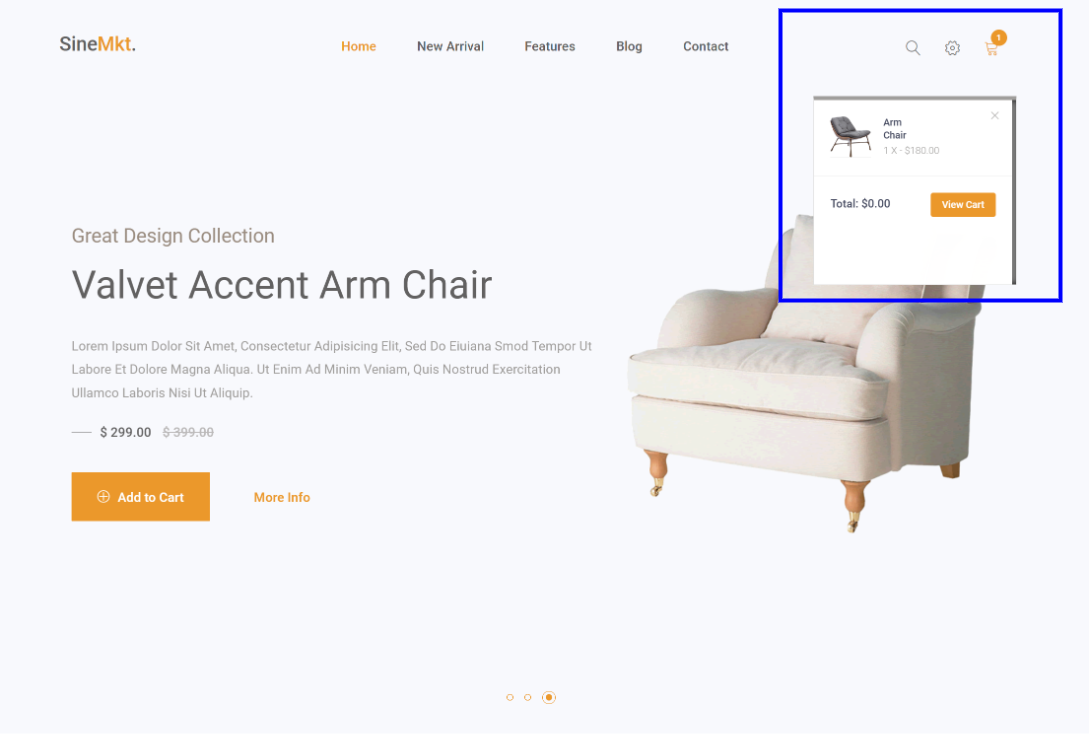
\includegraphics[width=0.9\textwidth]{picture/experiment/test-environment-no1.png}
    \caption{Hover購物車圖示後出現下拉示畫面之網頁變化}
    \label{f4.2}
\end{figure}

\subsection{案例二:點擊搜尋框後,僅需要了解該元件屬性變化}\label{s4.2.2}
\indent
實驗人員的測試情境為點擊搜尋圖標後,將隱藏的搜尋框展開,
並找出有因為此互動而有變化的元件,如圖\ref{f4.3}所示。
該案例需要找出一個指定元件的屬性變化,如果實驗人員皆找出變化並指出在Dev Tools中的位置則計為成功並記錄秒數。
在此情境中,實驗人員可以使用擴充元件中``Only display change of current selecting element''的Option,
讓實驗人員可以利用該Option過濾掉其餘畫面中不是搜尋框的變化,並指出在Dev Tools中的位置,讓實驗人員專注在指定元件的屬性中。

\begin{figure}[H]
    \centering
    \setlength{\abovecaptionskip}{-5pt}
    \setlength{\belowcaptionskip}{0pt}
    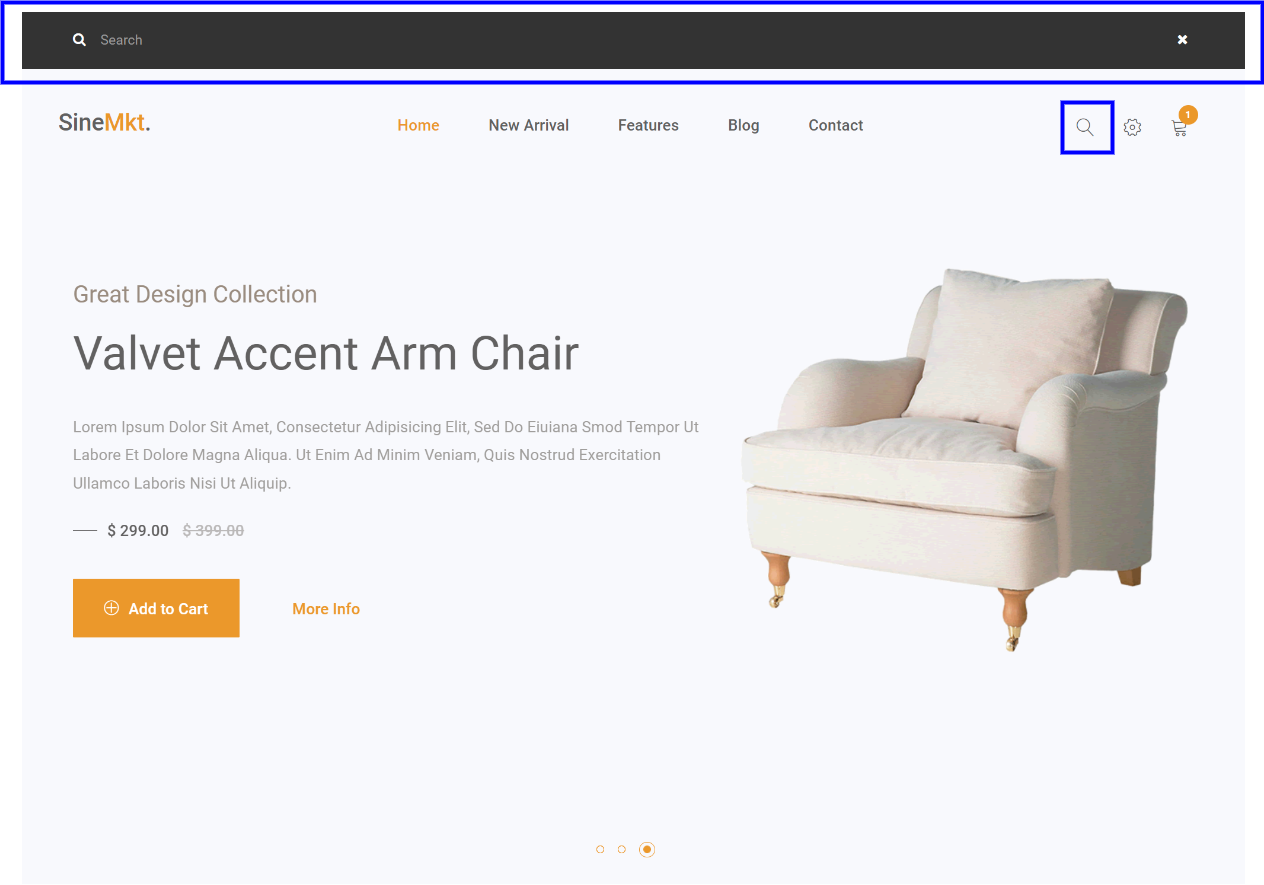
\includegraphics[width=0.9\textwidth]{picture/experiment/test-environment-no2.png}
    \caption{點擊搜尋圖標後之網頁變化}
    \label{f4.3}
\end{figure}

\subsection{案例三:網頁中畫面定時更換內容}\label{s4.2.3}
\indent
實驗人員的測試情境為在網頁中的產品促銷頁面更換的情況下,
找出因為畫面更換而屬性出現變化的元件。
在此產品促銷頁面中,有三個子頁面,裡面各有一個促銷商品。
若實驗人員的滑鼠鼠標沒有在促銷頁面上,
它會定時切換至不同的頁面中,
實驗人員可以在不用操作頁面的情況下,
看到每個在頁面上的促銷商品,
也可以點擊下方的小圓點手動切換畫面,
如圖\ref{f4.4}所示。

該案例需要找出四個元件的屬性變化,如果實驗人員皆找出變化並指出在Dev Tools中的位置則計為成功並記錄秒數。

\begin{figure}[H]
    \centering
    \setlength{\abovecaptionskip}{-5pt}
    \setlength{\belowcaptionskip}{0pt}
    \includegraphics[width=0.9\textwidth]{picture/experiment/test-environment-no3.png}
    \caption{產品促銷頁面循環示意圖}
    \label{f4.4}
\end{figure}


\subsection{案例四:點擊上方導覽列跳轉到該類別畫面}\label{s4.2.4}
\indent
實驗人員的測試情境為點擊網頁上方的導覽列,
可以快速跳轉到該網頁的指定區塊,
讓實驗人員不用花費多餘的時間尋找該區塊在頁面中的位置,如圖\ref{f4.5}所示。
一般在畫面快速跳轉的情況下,
無法快速地知道那些元件屬性有改變到,
且必須要從整個網頁中慢慢尋找,
透過此工具,
可以快速地呈現差異結果提供給實驗人員判斷是否適合當XPath表達式的條件。
該案例需要找出四個元件的屬性變化,
如果實驗人員皆找出變化並指出在Dev Tools中的位置則計為成功並記錄秒數。

\begin{figure}[H]
    \centering
    \setlength{\abovecaptionskip}{-5pt}
    \setlength{\belowcaptionskip}{0pt}
    \includegraphics[width=0.6\textwidth]{picture/experiment/test-environment-no4.png}
    \caption{利用導覽列跳轉到其他畫面之示意圖}
    \label{f4.5}
\end{figure}

\subsection{案例五:互動後當下網頁畫面無變化}\label{s4.2.5}
\indent
實驗人員的使用情境為點擊促銷頁面中的按鈕後,網頁下方標題``New Arrivals''下方會多一排文字。
正常狀況下,
在點擊按鈕時,標題``New Arrivals''是沒有在畫面中的,
導致實驗人員在點擊後看不到網站的變化。
因為產生變化的元件沒有在畫面中,
無法使用Developer Tools中``Inspect Element''的功能定位到該元件附近,
在未展開元件的情況下,也無法看見紫色漸淡背景框,
實驗人員只能上下滑動頁面觀察網頁畫面的變化來找出新增的元件,如圖\ref{f4.5}所示。
該案例需要找出一個被添加的元件,如果實驗人員找出變化並指出在Develope Tool中的位置則計為成功並記錄秒數。

\begin{figure}[H]
    \centering
    \setlength{\abovecaptionskip}{-5pt}
    \setlength{\belowcaptionskip}{0pt}
    \includegraphics[width=1.0\textwidth]{picture/experiment/test-environment-no5.png}
    \caption{當下網頁中無包括有變化的元件之示意圖}
    \label{f4.6}
\end{figure}

\newpage

\section{實驗數據分析}\label{s4.3}
\indent
本次實驗共有14位實驗人員參與,分成無相關經驗的7位以及有相關經驗的7位,藉由實驗人員的操作時間來比較有無使用此工具之差別。
表\ref{t4.1}、\ref{t4.2}使用的A符號,代表是無使用擴充程式的情況下;使用的B符號,代表是有使用擴充程式的情況下。

\subsection{無相關經驗實驗人員實例操作時間比較}\label{s4.3.1}
表\ref{t4.1}為紀錄無相關經驗的實驗人員在不同的實例下,分別使用兩種不同的尋找XPath路徑條件方法來比較其花費的時間,
從表中可見每一位實驗者大部分的實例是使用擴充工具會有明顯的改善,極少數會有使用擴充工具較慢的情況。
但從圖\ref{f4.7}可以明顯看出在五個案例的平均數據中,
使用擴充工具所花費的時間有明顯的降低,
減少的時間達25\%以上,案例五甚至有高達70\%左右。

\begin{table}[H]
    \begin{center}
    \setlength{\abovecaptionskip}{10pt}
    \setlength{\belowcaptionskip}{-10pt}
    \caption{無相關經驗的實驗人員在有無使用擴充工具的情況下比較五個實例操作時間}\label{t4.1}
        \begin{tabular}{|c|c|c|c|c|c|c|c|c|}   \hline
        & 人員1   & 人員2   & 人員3   & 人員4   & 人員5   & 人員6   & 人員7    & \textbf{平均時間}\\\hline\hline
        實例一 [A]   & 02m34s    & 02m14s    & 01m24s    & 02m58s    & 01m32s    & 02m07s    & 03m17s    & \textbf{02m18s}\\\hline
        實例一 [B]   & 02m10s    & 01m50s    & 01m15s    & 02m13s    & 00m38s    & 01m37s    & 02m03s    & \textbf{01m41s}\\\hline\hline
        實例二 [A]   & 04m38s    & 01m36s    & 00m41s    & 01m19s    & 01m12s    & 02m38s    & 01m22s    & \textbf{01m55s}\\\hline
        實例二 [B]   & 01m03s    & 00m54s    & 00m56s    & 01m05s    & 00m53s    & 01m07s    & 00m58s    & \textbf{00m59s}\\\hline\hline
        實例三 [A]   & 03m06s    & 03m36s    & 03m09s    & 04m38s    & 00m53s    & 03m30s    & 03m26s    & \textbf{03m11s}\\\hline
        實例三 [B]   & 01m21s    & 03m11s    & 01m23s    & 02m50s    & 01m15s    & 01m15s    & 02m36s    & \textbf{01m59s}\\\hline\hline
        實例四 [A]   & 03m28s    & 03m19s    & 02m45s    & 02m30s    & 02m47s    & 03m52s    & 04m03s    & \textbf{03m15s}\\\hline
        實例四 [B]   & 01m37s    & 02m11s    & 01m31s    & 02m57s    & 01m37s    & 02m51s    & 02m38s    & \textbf{02m12s}\\\hline\hline
        實例五 [A]   & 04m20s    & 02m51s    & 02m30s    & 04m16s    & 03m01s    & 01m43s    & 01m05s    & \textbf{02m49s}\\\hline
        實例五 [B]   & 01m26s    & 00m38s    & 00m32s    & 01m19s    & 00m30s    & 00m31s    & 00m35s    & \textbf{00m47s}\\\hline\hline
        \end{tabular}
    \end{center}
\end{table}

\begin{figure}[H]
    \centering
    \setlength{\abovecaptionskip}{-15pt}
    \setlength{\belowcaptionskip}{0pt}
    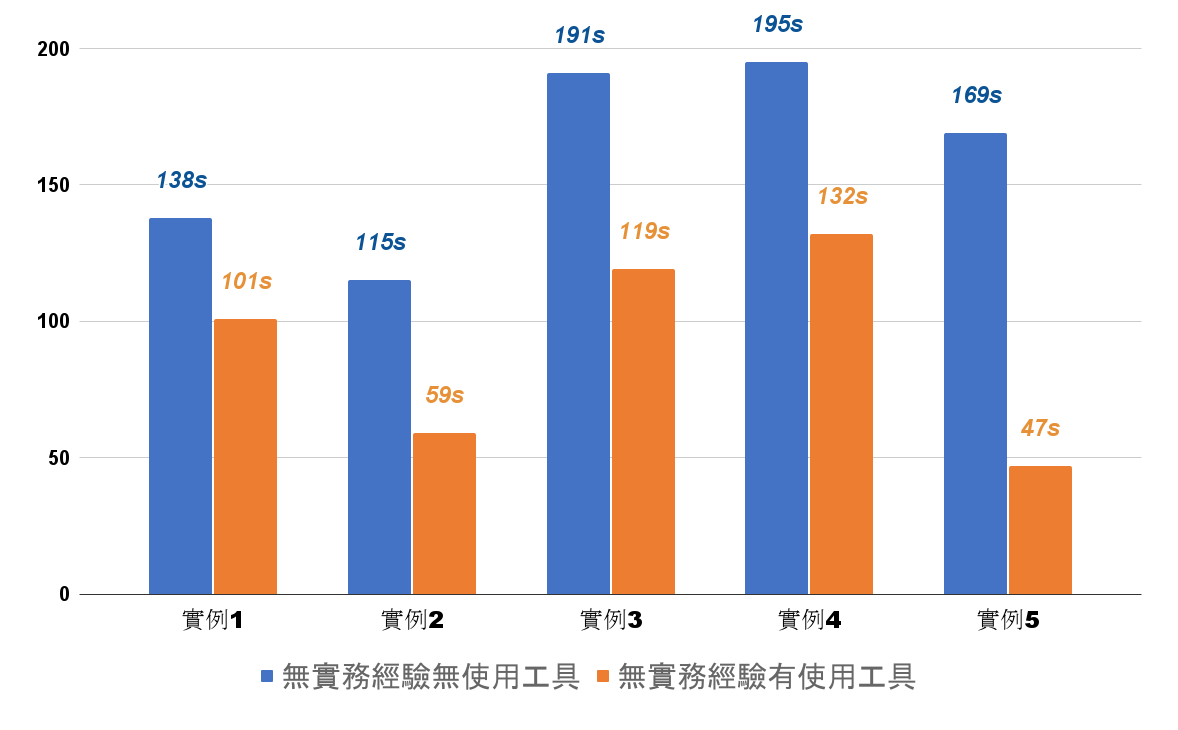
\includegraphics[width=0.87\textwidth]{picture/experiment/ch4-no_experience_compare.png}
    \caption{無相關經驗有無使用工具之比較(單位:秒)}
    \label{f4.7}
\end{figure}

\subsection{有相關經驗實驗人員實例操作時間比較}\label{s4.3.2}
表\ref{t4.2}為紀錄有相關經驗的實驗人員在各個實例下使用兩種不同尋找XPath的方法之比較其花費的時間,
從表中可以發現,相較於無相關經驗的實驗人員,有相關經驗的實驗人員有無使用擴充工具的時間差異不大,甚至有時候會略慢。
在實驗的過程中有發現,在使用工具時,雖然可以快速找到變化,但無法快速找到變化元件的HTML位置,在章節\ref{s5.2.2}會對此情況探討,
但從圖\ref{f4.8}可以發現,
案例二雖然平均時間相近,
但案例二的實作過程只要找尋一個元件的變化,
有相關經驗的實驗人員平時在找尋條件時也都只會看當下的元件,若當下的元件沒有複雜且快速的變化,使用工具對當下的情境是不會特別有幫助的,所以案例二的結果是可以預期的。
雖然使用工具依然可以減少約20\%的花費時間,但減少的時間不如無相關經驗的實驗人員明顯。

\begin{table}[H]
    \begin{center}
    \setlength{\abovecaptionskip}{10pt}
    \setlength{\belowcaptionskip}{-10pt}
    
    \caption{有相關經驗的實驗人員在有無使用擴充工具的情況下比較五個實例操作時間}\label{t4.2}
        \begin{tabular}{|c|c|c|c|c|c|c|c|c|}   \hline
        & 人員1   & 人員2   & 人員3   & 人員4   & 人員5   & 人員6   & 人員7    & \textbf{平均時間}\\\hline\hline
        實例一 [A]   & 01m16s    & 02m17s    & 02m28s    & 02m19s    & 02m04s    & 02m11s    & 02m41s    & \textbf{02m11s}\\\hline
        實例一 [B]   & 00m58s    & 01m43s    & 01m50s    & 01m56s    & 01m36s    & 02m01s    & 02m49s    & \textbf{01m50s}\\\hline\hline
        實例二 [A]   & 01m10s    & 01m53s    & 01m17s    & 01m16s    & 00m58s    & 00m44s    & 01m19s    & \textbf{01m14s}\\\hline
        實例二 [B]   & 00m51s    & 01m40s    & 01m25s    & 00m59s    & 00m46s    & 01m00s    & 01m22s    & \textbf{01m09s}\\\hline\hline
        實例三 [A]   & 03m28s    & 02m12s    & 02m00s    & 04m20s    & 01m50s    & 01m22s    & 03m26s    & \textbf{02m40s}\\\hline
        實例三 [B]   & 01m24s    & 03m20s    & 01m20s    & 01m38s    & 01m09s    & 01m24s    & 02m57s    & \textbf{01m53s}\\\hline\hline
        實例四 [A]   & 02m40s    & 02m44s    & 02m40s    & 01m56s    & 02m15s    & 01m53s    & 02m30s    & \textbf{02m23s}\\\hline
        實例四 [B]   & 01m20s    & 01m52s    & 01m33s    & 01m27s    & 01m40s    & 01m10s    & 02m31s    & \textbf{01m39s}\\\hline\hline
        實例五 [A]   & 04m48s    & 02m26s    & 04m41s    & 02m29s    & 01m58s    & 01m53s    & 01m20s    & \textbf{02m48s}\\\hline
        實例五 [B]   & 00m30s    & 01m07s    & 00m47s    & 00m32s    & 00m27s    & 00m39s    & 00m37s    & \textbf{00m40s}\\\hline\hline
        \end{tabular}
    \end{center}
\end{table}

\begin{figure}[H]
    \centering
    \setlength{\abovecaptionskip}{-15pt}
    \setlength{\belowcaptionskip}{0pt}
    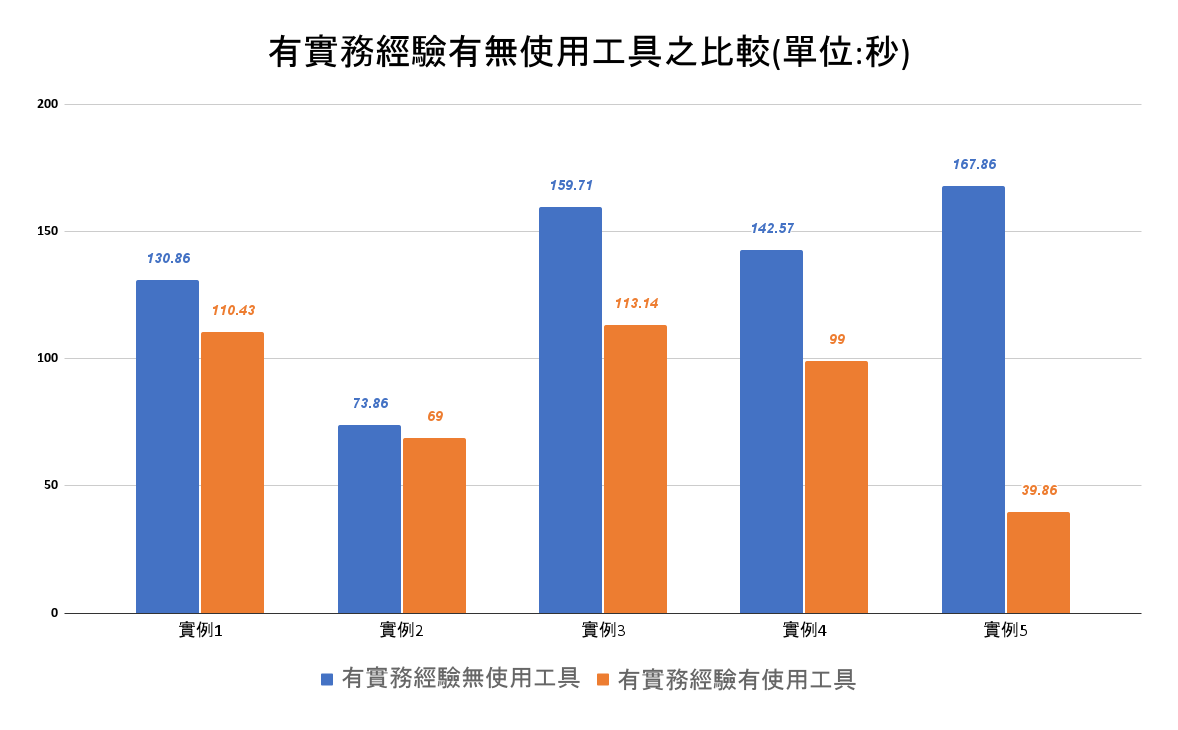
\includegraphics[width=0.87\textwidth]{picture/experiment/ch4-have_experience_compare.png}
    \caption{有相關經驗有無使用工具之比較(單位:秒)}
    \label{f4.8}
\end{figure}

\subsection{全體實驗人員實例操作時間比較}\label{s4.3.3}

由圖\ref{f4.9}的全部實驗人員平均時間統計結果,可以看出每個案例都減少$20\%\sim30\%$的時間,
其中案例五在有經驗或無經驗的情況下,使用擴充程式能使找尋變化的時間皆大幅減少,
由此可以看出即使有經驗的實驗人員,也較難找出超出畫面外的元件變化。

% \begin{table}[H]
%     \begin{center}
%     \setlength{\abovecaptionskip}{10pt}
%     \setlength{\belowcaptionskip}{15pt}
%     \caption{在無實務經驗情況下,是否使用擴充工具之五個實例操作時間比較}\label{t4.3}
%         \begin{tabular}{|c|c|c|c|}   \hline
%         & 無實務經驗人員平均   & 有實務經驗人員平均   & \textbf{總人員平均}\\\hline
%         實例一 [A]   & 02m18s   & 02m11s    & \textbf{02m14s}\\\hline
%         實例一 [B]   & 01m41s   & 01m50s    & \textbf{01m46s}\\\hline
%         實例二 [A]   & 01m55s   & 01m14s    & \textbf{01m35s}\\\hline
%         實例二 [B]   & 00m59s   & 01m09s    & \textbf{01m04s}\\\hline
%         實例三 [A]   & 03m11s   & 02m40s    & \textbf{02m55s}\\\hline
%         實例三 [B]   & 01m59s   & 01m53s    & \textbf{01m56s}\\\hline
%         實例四 [A]   & 03m15s   & 02m23s    & \textbf{02m49s}\\\hline
%         實例四 [B]   & 02m12s   & 01m39s    & \textbf{01m55s}\\\hline
%         實例五 [A]   & 02m49s   & 02m48s    & \textbf{02m49s}\\\hline
%         實例五 [B]   & 00m47s   & 00m40s    & \textbf{00m44s}\\\hline
%         \end{tabular}
%     \end{center}
% \end{table}

\begin{figure}[H]
    \centering
    \setlength{\abovecaptionskip}{-15pt}
    \setlength{\belowcaptionskip}{0pt}
    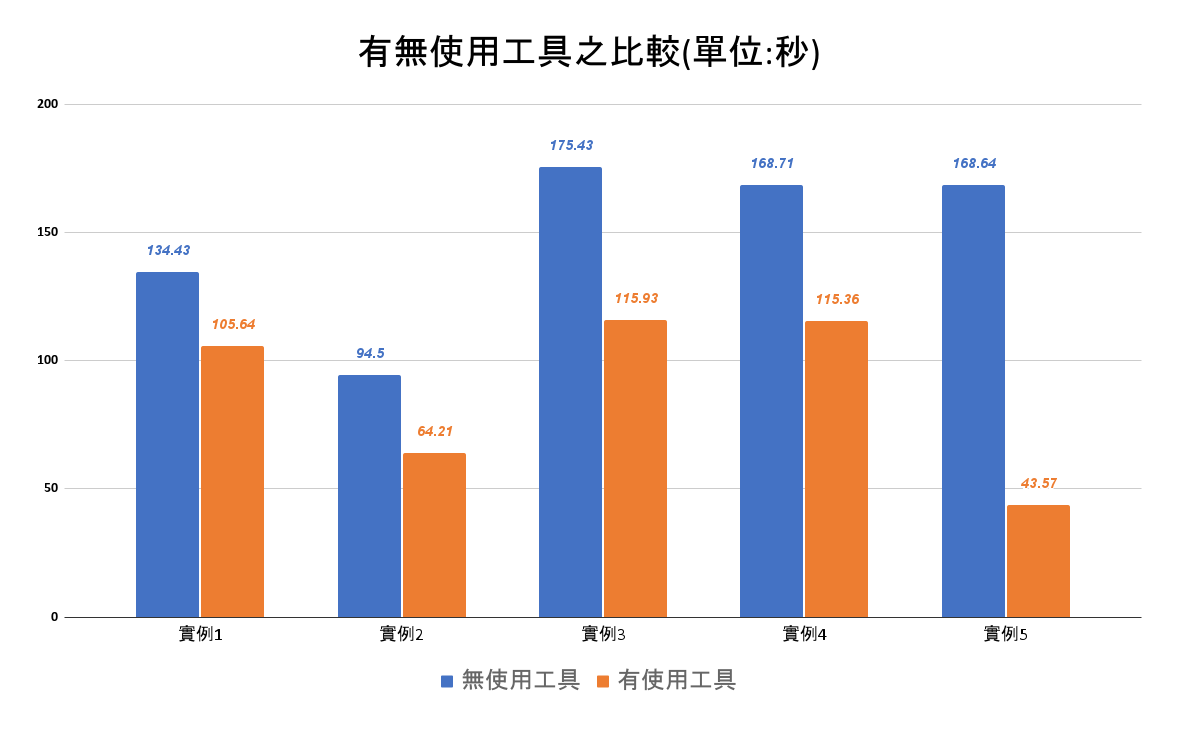
\includegraphics[width=0.87\textwidth]{picture/experiment/ch4-all_compare.png}
    \caption{有無使用工具之比較(單位:秒)}
    \label{f4.9}
\end{figure}


% \begin{table}[H]
%     \begin{center}
%     \setlength{\abovecaptionskip}{10pt}
%     \setlength{\belowcaptionskip}{20pt}
%     \caption{有相關經驗的情況下,是否使用擴充工具之五個實例操作時間比較}\label{t4.2}
%         \begin{tabular}{|c|c|c|c|c|c|c|c|}   \hline
%         & 人員1   & 人員2   & 人員3   & 人員4   & 人員5   & 人員6   & 人員7\\\hline
%         \makecell[l]{實例一 \\ (無使用擴充元件)}  & 06m02s    & 03m24s    & 04m20s    & 04m20s    & 04m20s    & 04m20s    & 04m20s    \\\hline
%         實例一 A  & 06m02s    & 03m24s    & 04m20s    & 04m20s    & 04m20s    & 04m20s    & 04m20s    \\\hline
%         1A  & 06m02s    & 03m24s    & 04m20s    & 04m20s    & 04m20s    & 04m20s    & 04m20s    \\\hline
%         1B  & 06m02s    & 03m24s    & 04m20s    & 04m20s    & 04m20s    & 04m20s    & 04m20s    \\\hline
%         \textbf{增減時間}    & \textbf{06m18s}    & \textbf{04m38s}    & \textbf{06m18s}    & \textbf{06m18s}    & \textbf{06m18s}    & \textbf{06m18s}    & \textbf{06m18s}    \\\hline
%         \textbf{增減比例}    & \textbf{06m18s}    & \textbf{04m38s}    & \textbf{06m18s}    & \textbf{06m18s}    & \textbf{06m18s}    & \textbf{06m18s}    & \textbf{06m18s}    \\\hline
%         \end{tabular}
%     \end{center}
% \end{table}